\section{Evaluation}
\label{sec:evaluation}

We compare HStore with HyperGraphDB, the only other embedded store we know of whose atoms are hyperedges with a variable number of members. The evaluation asks four questions. How do the two systems compare on reads, writes and space when the data fits in the cache and when it does not (\cref{sec:eval-throughput,sec:eval-resources})? What do commits and reads cost one at a time, and how do reads behave while a writer is committing (\cref{sec:eval-latency})? How do the systems recover from a crash and reclaim space after deletes (\cref{sec:eval-space})? And how much does each of HStore's main design decisions contribute (\cref{sec:eval-ablation})?

\subsection{Setup}
\label{sec:eval-setup}

\paragraph{Dataset.} The dataset is generated from a fixed seed, so both systems load the same hypergraph. At scale $s$ it has $50{,}000\,s$ nodes and $100{,}000\,s$ hyperedges. A hyperedge starts with two members and gains each further member with probability 0.62, up to 32, for a mean cardinality of 3.6. Members are drawn as $\lfloor n u^{2.2}\rfloor$ for uniform $u\in[0,1)$ over $n$ nodes, so low-numbered nodes become hubs. At scale~1 half of the nodes are in at most 5 hyperedges, 370 are in more than 48, and the largest is in 2,645; at scale~4 the largest is in 5,714. Probe sets from the same seed select 100,000 random atoms, 20,000 pairs of nodes that share a hyperedge, and 20,000 node updates. A churn set selects 20\% of the hyperedges for deletion and 20,000 other hyperedges, each losing one member.

\paragraph{Workloads.} \Cref{tab:workloads} lists the \M{workloadCount} workloads, which run in this order in one process per system and run. Each adapter uses the plain storage API of its system: long ids and \code{forEachIncidentEdge}, \code{forEachMemberId} and \code{Writer.set} for HStore, persistent handles and \code{getIncidenceSet}, \code{getTargetAt} and \code{graph.replace} for HyperGraphDB. We do not use HyperGraphDB's traversal framework, so that both sides measure storage. HyperGraphDB links are immutable, so removing a member replaces the link. Every read and delete workload returns a checksum, such as the number of ids visited, and both systems returned the same checksum in every run.

\begin{table}[t]
\centering\footnotesize
\caption{Workloads, in execution order.}
\label{tab:workloads}
\begin{tabularx}{\columnwidth}{@{}lX@{}}
\toprule
Workload & Operation \\
\midrule
\wl{ingest.nodes}, \wl{.edges} & insert all nodes, then all hyperedges, 1,000 per transaction \\
\wl{read.incidence} & list the hyperedges that contain a node; 100,000 probes \\
\wl{read.members} & list a hyperedge's members; 100,000 probes \\
\wl{read.comembership} & count the hyperedges that contain both nodes of a pair \\
\wl{read.twohop} & count distinct nodes that share a hyperedge with a node \\
\wl{read.incidence.parallel} & \wl{read.incidence} from 8 threads \\
\wl{latency.read} & one incidence lookup per read transaction, each timed \\
\wl{write.update} & replace a node's value; 20,000 updates, 1,000 per transaction \\
\wl{latency.commit} & one update per transaction, each timed; 5,000 commits \\
\wl{mixed.read}, \wl{.write} & 7 reader threads for 10\,s beside a writer committing 10 updates per transaction on a fixed schedule of 1,000 updates/s \\
\wl{large.*} & create one hyperedge that contains every node, scan it 400 times, probe it 100,000 times \\
\wl{reopen} & close cleanly and open again \\
\wl{read.incidence.cold} & \wl{read.incidence} right after the reopen \\
\wl{churn.delete}, \wl{.remove} & delete 20\% of the hyperedges; remove one member from 20,000 others \\
\wl{compaction} & single-update commits at 50/s while a full space reclamation runs \\
\wl{disk}, \wl{.churned}, \wl{.compacted} & bytes on disk after load, after the deletes, after reclamation \\
\wl{recover} & open a store whose ingest process was killed with SIGKILL \\
\bottomrule
\end{tabularx}
\end{table}

\paragraph{Measurement.} Throughput is the operation count divided by the elapsed time of the whole operation set. Each write workload ends with a flush outside the timed section (an HStore checkpoint or a JE \code{sync}), so bytes still in buffers are charged to the workload that produced them. Every read workload except \wl{read.incidence.cold} first runs untimed for at least 2\,s, so both systems are measured with their read paths compiled by the JIT. The latency workloads time every transaction; in \wl{mixed} and \wl{compaction} the writer follows a fixed schedule and its latency is measured from the scheduled start, so a stall is charged to every commit queued behind it~\cite{fair-benchmarking}. Both systems count their own file I/O: HStore its log and page bytes, including pages moved by compaction, and HyperGraphDB the bytes JE writes and reads, including its cleaner. Allocation per operation comes from the JVM's per-thread allocation counters and the retained heap from a full collection after ingest.

\paragraph{Configurations.} We run three configurations. S1~async is scale~1 with asynchronous commits. S1~sync is scale~1 with synchronous commits. S4~async is scale~4 with asynchronous commits; there the files of both systems are larger than their 64\,MiB caches. Both caches get the same 64\,MiB budget. HStore's covers decoded nodes; JE's covers its B+tree nodes and records, and HyperGraphDB's atom cache comes on top and cannot be capped in bytes. HyperGraphDB~1.4 begins every JE transaction with \code{WRITE\_NO\_SYNC}, which overrides the environment's \code{COMMIT\_SYNC}; under S1~sync its adapter therefore forces JE's log after every commit, which is what \code{COMMIT\_SYNC} would do.

\paragraph{Machine.} All runs used one Azure \code{Standard\_D8ds\_v5} virtual machine: four cores (eight hardware threads) of an Intel Xeon Platinum 8370C at 2.8\,GHz, 32\,GiB of memory, and Ubuntu 24.04 with Linux 6.17. Both systems kept their files on the machine's local 300\,GB temporary SSD, formatted as ext4, and ran on Oracle GraalVM 25.0.4 in JVM mode. HyperGraphDB is version 1.4 built from commit \code{99485a1} with Berkeley DB JE 5.0.73, the JE version its storage module is written against. Each system runs in its own JVM with a fixed 4\,GiB heap and the Parallel collector. Runs alternate between the two systems, so that a slow period on the machine affects both. We report medians over \M{runss1async}, \M{runss1sync} and \M{runss4async} runs per system for the three configurations. A ratio is oriented so that values above 1 favour HStore, and it is marked with $\dagger$ when the ranges of the two systems' runs overlap.

\begin{table*}[t]
\centering\footnotesize
\caption{Median results. Rates are operations per second; \wl{disk} rows are bytes on disk; \wl{reopen} and \wl{recover} are times. A ratio above 1 favours HStore, and $\dagger$ marks a ratio whose run ranges overlap. The S1~sync column gives only the ratio; its rates differ from S1~async only for the commit-bound workloads discussed in the text.}
\label{tab:results}
\begin{tabular}{@{}lrrrrrrr@{}}
\toprule
& \multicolumn{3}{c}{S1 async} & S1 sync & \multicolumn{3}{c}{S4 async} \\
\cmidrule(lr){2-4}\cmidrule(lr){5-5}\cmidrule(l){6-8}
Workload & HStore & HyperGraphDB & ratio & ratio & HStore & HyperGraphDB & ratio \\
\midrule
\wl{ingest.nodes} & 33.3\,k & 19.6\,k & 1.7 & 1.7 & 42.9\,k & 24.0\,k & 1.8 \\
\wl{ingest.edges} & 28.9\,k & 21.3\,k & 1.4 & 1.3 & 21.5\,k & 2.71\,k & 7.9 \\
\wl{read.incidence} & 3.10\,M & 1.25\,M & 2.5 & 3.1 & 2.62\,M & 1.11\,M & 2.4 \\
\wl{read.members} & 2.29\,M & 1.66\,M & 1.4 & 1.6 & 2.13\,M & 1.27\,M & 1.7 \\
\wl{read.comembership} & 272\,k & 49.8\,k & 5.5 & 4.9 & 281\,k & 41.4\,k & 6.8 \\
\wl{read.twohop} & 243\,k & 83.6\,k & 2.9 & 3.4 & 172\,k & 80.9\,k & 2.1 \\
\wl{read.incidence.parallel} & 14.1\,M & 1.28\,M & 11 & 12.8 & 8.21\,M & 1.26\,M & 6.5 \\
\wl{latency.read} & 2.07\,M & 505\,k & 4.1 & 3.8 & 1.79\,M & 470\,k & 3.8 \\
\wl{write.update} & 40.9\,k & 7.26\,k & 5.6 & 5.8 & 30.2\,k & 2.47\,k & 12.2 \\
\wl{latency.commit} & 6.96\,k & 7.33\,k & 0.95$^\dagger$ & 1.2 & 10.1\,k & 2.54\,k & 4.0 \\
\wl{mixed.read} & 8.73\,M & 1.13\,M & 7.7 & 8.0 & 8.55\,M & 1.11\,M & 7.7 \\
\wl{mixed.write} & 1,000 & 1,000 & 1.0 & 1.0 & 1,000 & 999 & 1.0 \\
\wl{large.ingest} & 431\,k & 47.6\,k & 9.1 & 7.4 & 489\,k & 13.6\,k & 36.1 \\
\wl{large.scan} & 1,668\,M & 344\,M & 4.8 & 4.5 & 1,583\,M & 358\,M & 4.4 \\
\wl{large.probe} & 6.60\,M & 1.01\,M & 6.5 & 7.2 & 5.61\,M & 844\,k & 6.7 \\
\wl{reopen} & 78.5\,ms & 978\,ms & 12.5 & 13 & 92.9\,ms & 1,279\,ms & 13.8 \\
\wl{read.incidence.cold} & 1.73\,M & 67.6\,k & 25.6 & 28.1 & 1.23\,M & 15.1\,k & 81.6 \\
\wl{disk} & 85.7\,MiB & 400\,MiB & 4.7 & 4.3 & 172\,MiB & 2.30\,GiB & 13.7 \\
\wl{churn.delete} & 16.1\,k & 5.18\,k & 3.1 & 2.9 & 2.64\,k & 1.99\,k & 1.3 \\
\wl{churn.remove} & 23.1\,k & 10.7\,k & 2.2 & 2.1 & 4.08\,k & 3.53\,k & 1.2 \\
\wl{read.incidence.churned} & 3.10\,M & 1.30\,M & 2.4 & 2.6 & 2.75\,M & 1.05\,M & 2.6 \\
\wl{disk.churned} & 116\,MiB & 293\,MiB & 2.5 & 2.0 & 1.14\,GiB & 1.91\,GiB & 1.7 \\
\wl{compaction.baseline} & 50.1 & 50.1 & 1.0$^\dagger$ & 1.0$^\dagger$ & 50.1 & 50.1 & 1.0 \\
\wl{compaction} & 50.1 & 50.1 & 1.0$^\dagger$ & 1.0$^\dagger$ & 50.1 & 50.0 & 1.0 \\
\wl{disk.compacted} & 93.3\,MiB & 234\,MiB & 2.5 & 2.7 & 183\,MiB & 1.15\,GiB & 6.4 \\
\wl{recover} & 84.8\,ms & 113\,ms & 1.3$^\dagger$ & 1.4 & 162\,ms & 449\,ms & 2.8 \\
\bottomrule

\end{tabular}
\end{table*}

\begin{figure}[t]
\centering
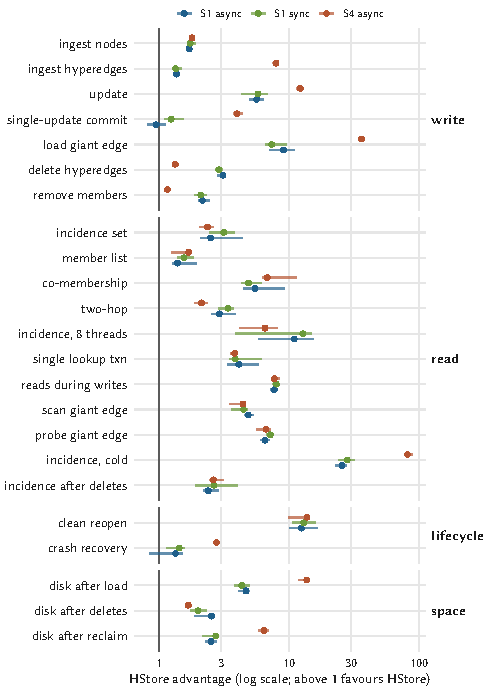
\includegraphics[width=\columnwidth]{figures/ratios}
\caption{HStore's advantage per workload and configuration: the ratio of the medians, with a bar from the least to the most favourable pairing of runs. Workloads with a fixed rate are left out.}
\label{fig:ratios}
\end{figure}

\subsection{Throughput}
\label{sec:eval-throughput}

\Cref{tab:results} lists every median and \cref{fig:ratios} plots the ratios. Every read and delete workload returned the same checksum on both systems in every run. HStore is ahead on every workload whose rate the harness does not fix, with one exception: single-update commits under asynchronous durability at scale~1, where the two systems are within each other's range (\M{ratios1asynclatencycommit}).

\paragraph{Reads.} A batch of incidence lookups is \M{ratios1asyncreadincidence} times faster at scale~1 and \M{ratios4asyncreadincidence} times faster at scale~4, and member lookups are \M{ratios1asyncreadmembers} and \M{ratios4asyncreadmembers} times faster. Counting the hyperedges two nodes share is \M{ratios1asyncreadcomembership} times faster at scale~1. HStore answers it by intersecting the two incidence trees and skipping every pair of subtrees whose key ranges do not overlap; HyperGraphDB evaluates the conjunction of two incidence conditions. From eight threads HStore reaches \M{hss1asyncreadincidenceparallel} incidence lookups per second at scale~1, while HyperGraphDB stays at \M{hgs1asyncreadincidenceparallel}, about its single-thread rate of \M{hgs1asyncreadincidence}. Right after a reopen the gap is widest: \M{ratios1asyncreadincidencecold} times at scale~1 and \M{ratios4asyncreadincidencecold} times at scale~4. HStore reads its segments through memory maps that the operating system's page cache still holds and decodes a leaf record only when it is read, while JE fills its own cache from its log one node at a time.

\paragraph{Writes.} Node and hyperedge ingest are \M{ratios1asyncingestnodes} and \M{ratios1asyncingestedges} times faster at scale~1. At scale~4, where both systems' files outgrow their 64\,MiB caches, hyperedge ingest is \M{ratios4asyncingestedges} times faster, because HyperGraphDB drops from \M{hgs1asyncingestedges} to \M{hgs4asyncingestedges} hyperedges per second. Updates in batches of 1,000 are \M{ratios1asyncwriteupdate} and \M{ratios4asyncwriteupdate} times faster. Creating one hyperedge that holds every node is \M{ratios1asynclargeingest} times faster at scale~1 and \M{ratios4asynclargeingest} times at scale~4, and scanning it is \M{ratios1asynclargescan} times faster. Deletes are the closest. At scale~4 HStore deletes \M{hss4asyncchurndelete} hyperedges per second, \M{ratios4asyncchurndelete} times HyperGraphDB's rate, against \M{ratios1asyncchurndelete} times at scale~1. Deleting a hyperedge removes it from the reverse index of every member, and at scale~4 those postings are spread over many more pages than the cache holds.

\paragraph{Opening a database.} A clean reopen takes \M{hss1asyncreopen} against \M{hgs1asyncreopen} at scale~1 (\M{ratios1asyncreopen} times faster). HStore loads the catalog image and maps the segments; nothing is replayed after a clean shutdown.

\subsection{Latency}
\label{sec:eval-latency}

\begin{figure*}[t]
\centering
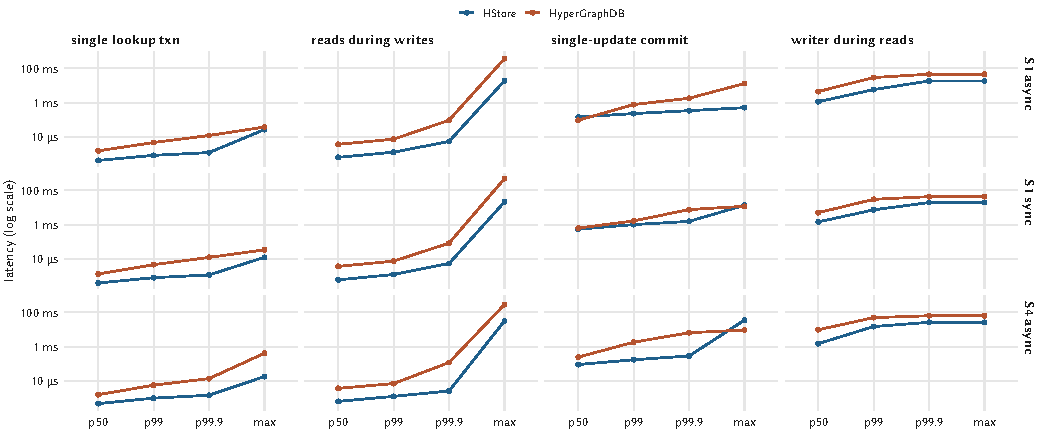
\includegraphics[width=\textwidth]{figures/latency}
\caption{Latency percentiles, medians over runs. Read latencies are per transaction with one lookup; commit latencies include the wait for the group commit; in the mixed workload the writer's latency is measured from each transaction's scheduled start.}
\label{fig:latency}
\end{figure*}

\Cref{fig:latency} shows the percentiles. A read transaction that looks up one incidence set takes \M{lats1asynclatencyreadhspfifty} at the median on HStore and \M{lats1asynclatencyreadhgpfifty} on HyperGraphDB, and \M{lats1asynclatencyreadhspninetyninenine} against \M{lats1asynclatencyreadhgpninetyninenine} at the 99.9th percentile.

Single-update commits are where the systems are closest. Under asynchronous durability at scale~1, HyperGraphDB's median commit is faster (\M{lats1asynclatencycommithgpfifty} against \M{lats1asynclatencycommithspfifty}), but its tail is longer: \M{lats1asynclatencycommithgpninetynine} against \M{lats1asynclatencycommithspninetynine} at the 99th percentile and \M{lats1asynclatencycommithgpninetyninenine} against \M{lats1asynclatencycommithspninetyninenine} at the 99.9th. Under synchronous durability every commit waits for an fsync, and HStore's median is \M{lats1synclatencycommithspfifty} against \M{lats1synclatencycommithgpfifty}; a commit writes \M{writtens1synclatencycommiths} to HStore's log and data files and \M{writtens1synclatencycommithg} to JE's. At scale~4 HStore's commits are faster at every percentile up to the 99.9th (\M{lats4asynclatencycommithspninetyninenine} against \M{lats4asynclatencycommithgpninetyninenine}), but its slowest commit in a run is slower: \M{lats4asynclatencycommithsmax} at the median of the runs against \M{lats4asynclatencycommithgmax}. We have not yet traced these single stalls.

The mixed workload runs seven readers for 10\,s beside a writer that commits 1,000 updates per second on a fixed schedule. Both writers kept the schedule. HStore's readers complete \M{ratios1asyncmixedread} times as many lookups, with a median latency of \M{lats1asyncmixedreadhspfifty} against \M{lats1asyncmixedreadhgpfifty} and a 99.9th percentile of \M{lats1asyncmixedreadhspninetyninenine} against \M{lats1asyncmixedreadhgpninetyninenine}. HStore readers never take a lock, so the writer does not slow them, and the writer in turn finishes its transactions sooner: its 99th percentile, measured from the scheduled start, is \M{lats1asyncmixedwritehspninetynine} against \M{lats1asyncmixedwritehgpninetynine}.

\subsection{Resources}
\label{sec:eval-resources}

\begin{figure*}[t]
\centering
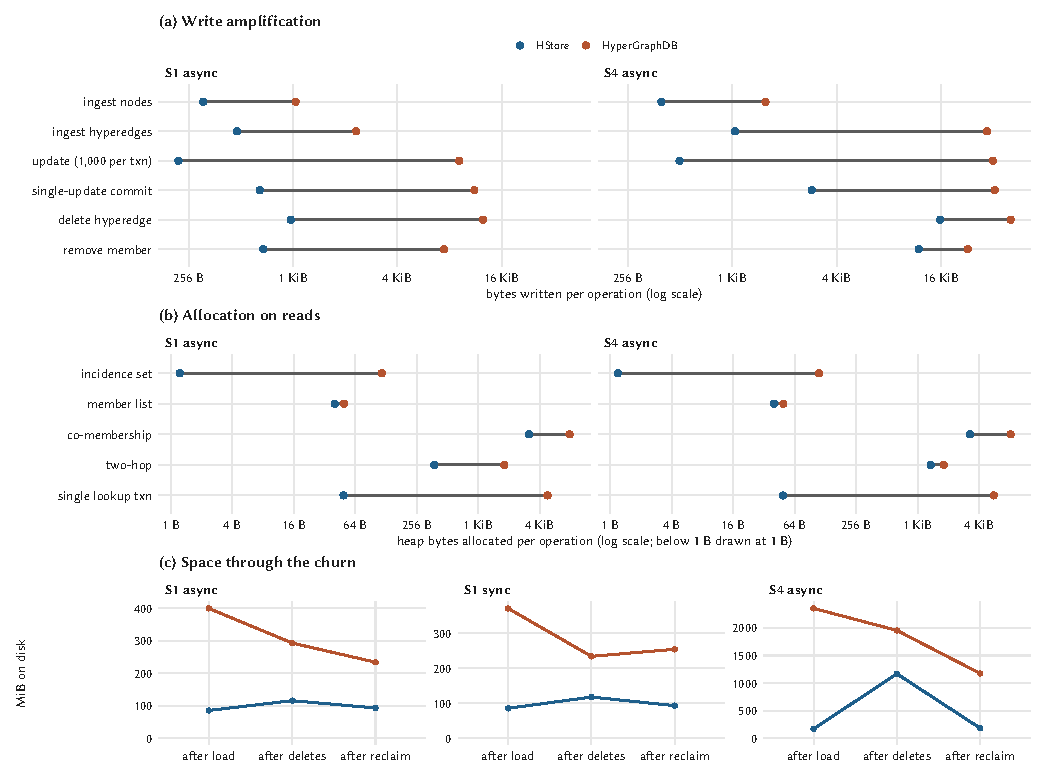
\includegraphics[width=\textwidth]{figures/resources}
\caption{(a) Bytes written to the log and data files per operation, including JE's cleaner and HStore's compaction. (b) Heap bytes allocated per operation on the read workloads, over all threads. (c) Bytes on disk after the load, after the deletes and after reclamation, each measured after a clean shutdown.}
\label{fig:resources}
\end{figure*}

\paragraph{Bytes written.} Logging keys instead of pages shows most clearly in the bytes written per change (\cref{fig:resources}a). An update in a batch writes \M{writtens1asyncwriteupdatehs} on HStore and \M{writtens1asyncwriteupdatehg} on HyperGraphDB, and a single-update commit \M{writtens1asynclatencycommiths} against \M{writtens1asynclatencycommithg}. At scale~4 hyperedge ingest writes \M{writtens4asyncingestedgeshs} per hyperedge against \M{writtens4asyncingestedgeshg}. Over a whole run at scale~4, HStore wrote \M{totalwrittens4asynchs} and HyperGraphDB \M{totalwrittens4asynchg}, \M{compactwrittens4asynchg} of it during the \wl{compaction} workload, while JE's cleaner copied live records out of old log files after the deletes.

\paragraph{Allocation and heap.} Reads on HStore allocate almost nothing (\cref{fig:resources}b): \M{allocs1asyncreadincidencehs} per incidence lookup in a batch against \M{allocs1asyncreadincidencehg}, and \M{allocs1asynclatencyreadhs} per single-lookup transaction against \M{allocs1asynclatencyreadhg}. In the mixed workload, where the readers allocate \M{allocs1asyncmixedreadhs} and \M{allocs1asyncmixedreadhg} per lookup, the collector spent \M{gcmss1asyncmixedreadhs} on HStore and \M{gcmss1asyncmixedreadhg} on HyperGraphDB over the 10\,s. HStore keeps more heap after ingest, \M{retaineds1asynchs} against \M{retaineds1asynchg} at scale~1 and \M{retaineds4asynchs} against \M{retaineds4asynchg} at scale~4. Both its node cache and its write buffer of nodes that no checkpoint has written yet are on the heap.

\subsection{Space and recovery}
\label{sec:eval-space}

After the load HStore's files take \M{hss1asyncdisk} at scale~1 and \M{hss4asyncdisk} at scale~4, against \M{hgs1asyncdisk} and \M{hgs4asyncdisk} for HyperGraphDB (\cref{fig:resources}c). The deletes grow HStore's files to \M{hss4asyncdiskchurned} at scale~4, because a page that a delete replaced stays until a checkpoint releases it and compaction empties its segment. HStore gives that space back on its own. The \wl{compaction} workload starts 10\,s later, after ten seconds of single-update commits with the background compactor running, and by then the files are back to \M{diskbeforecompacts4asynchs}; the explicit compaction that follows takes \M{compactmss4asynchs}. JE's cleaner, run until it reports nothing left to clean, takes \M{compactmss4asynchg} at scale~4. At scale~1 it usually takes well under a second, but one of the five runs took \M{compactmsmaxs1asynchg}. Commits continued on both systems while space was reclaimed and kept their schedule of 50 per second. After reclamation HStore's files are \M{hss1asyncdiskcompacted} and \M{hss4asyncdiskcompacted}, and HyperGraphDB's \M{hgs1asyncdiskcompacted} and \M{hgs4asyncdiskcompacted}.

In the \wl{recover} workload a child process ingests nodes in transactions of 1,000 and is killed with SIGKILL once half of them are acknowledged. No run of either system lost an acknowledged commit. Opening the killed store takes \M{hss1asyncrecover} on HStore and \M{hgs1asyncrecover} on HyperGraphDB at scale~1, and \M{hss4asyncrecover} against \M{hgs4asyncrecover} at scale~4. At scale~1 the child writes only a few megabytes of log before it is killed, so with the automatic threshold of \cref{sec:transactions} the open replays only the log written since the last background checkpoint.

\subsection{What each design choice contributes}
\label{sec:eval-ablation}

\begin{figure}[t]
\centering
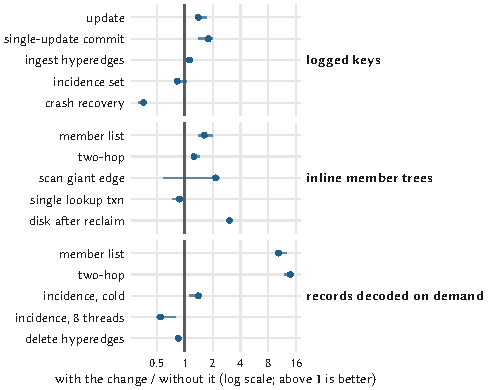
\includegraphics[width=\columnwidth]{figures/ablation}
\caption{Effect of three design choices, each measured on HStore alone at the commit that introduced it and at the commit before it. Logged keys and inline member trees run at scale~1, records decoded on demand at scale~4.}
\label{fig:ablation}
\end{figure}

To separate three of the decisions in \cref{sec:layout,sec:transactions}, we ran HStore alone at the commit that introduced each of them and at the commit just before it, with \M{ablrunslogical} runs of each build on the same machine (\cref{fig:ablation}). The two builds of a pair differ only in that change. Each pair comes from earlier in the project's history than the version measured above, so its absolute numbers are not comparable with \cref{tab:results}.

\paragraph{Logging keys instead of pages.} Before this change a commit wrote every new node from each changed leaf to the root. An update in a batch wrote \M{abllogicalwriteupdatewrittenbefore} before it and \M{abllogicalwriteupdatewrittenafter} after it, and a single-update commit \M{abllogicallatencycommitwrittenbefore} and \M{abllogicallatencycommitwrittenafter}. Batched updates became \M{abllogicalwriteupdate} times faster and single-update commits \M{abllogicallatencycommit} times faster. The cost is recovery. The open now replays the logged keys into the trees instead of finding pages already written, and opening the killed store took \M{abllogicalrecoverafter} instead of \M{abllogicalrecoverbefore}. The automatic checkpoint threshold, added later, bounds how much log the open has to replay. Most read workloads were 5 to 17\% slower after the change, two-hop queries excepted, and we have not investigated why.

\paragraph{Inline member trees.} Storing a small membership inside the hyperedge's record makes member lookups \M{ablinlinereadmembers} times faster and two-hop queries \M{ablinlinereadtwohop} times faster, because a lookup no longer follows a root reference to a tree of its own. It also removes a separate small leaf per hyperedge, and the files after reclamation shrink from \M{ablinlinediskcompactedbefore} to \M{ablinlinediskcompactedafter}. Single-lookup read transactions were slightly slower, at \M{ablinlinelatencyread} times their earlier rate.

\paragraph{Records decoded on demand.} With data larger than the cache, decoding a leaf record only when it is read makes member lookups \M{abllazyreadmembers} times faster (\M{abllazyreadmembersbefore} to \M{abllazyreadmembersafter} per second) and two-hop queries \M{abllazyreadtwohop} times faster, since a lookup that misses the cache decodes one record instead of a whole page. Incidence lookups right after a reopen gain \M{abllazyreadincidencecold} times. The same change cost almost half of the incidence rate from eight threads, from \M{abllazyreadincidenceparallelbefore} to \M{abllazyreadincidenceparallelafter} lookups per second, and deletes ran at \M{abllazychurndelete} times their earlier rate. We have not yet found what the eight readers contend on.

\subsection{Limits of this evaluation}

Both systems run on the JVM, on one machine, with one synthetic dataset. The dataset's skewed membership resembles real hypergraphs, but its hyperedges carry no properties beyond a name, and we did not test workloads with large property values or with many concurrent writers. HyperGraphDB is the only system we compare with, because it is the only embedded store we know of with first-class hyperedges, and its storage layer, JE~5.0.73, is more than a decade old. A comparison with a graph database storing reified hyperedges would answer a different question and is left for future work.
